\documentclass[11pt,a4paper]{article}
\usepackage[margin=2.3cm]{geometry}
\usepackage{amsmath,amssymb,amsfonts,booktabs}
\usepackage{graphicx}
\graphicspath{{./}{../}}
\usepackage[round]{natbib}
\usepackage[colorlinks=true,linkcolor=black,citecolor=black,urlcolor=blue]{hyperref}
\usepackage{setspace}
\setstretch{1.05}
\setlength{\parskip}{3pt}
\setlength{\parindent}{0pt}
\bibliographystyle{plainnat}

\newcommand{\hl}{\widehat{l}}

\title{\textbf{Peak Prediction Using Quantile Regression and Asymmetric Laplace Noise: Data-Driven Intervals for the Peak Location}}

% TODO: check author list, order and affiliations before submission
\author{
  Sa\"{i}d Maanan$^{1}$, Azzouz Dermoune$^{2}$, Daoud Ounaissi$^{3}$, Yousri Slaoui$^{4}$, Ahmed El Ghini$^{1}$\\[3pt]
  {\small $^{1}$LEAM, Mohammed V University in Rabat, Morocco\quad
  $^{2}$Laboratoire Paul Painlev\'e, USTL--CNRS--UMR 8524, Lille, France}\\
  {\small $^{3}$ESA, Angers, France\quad
  $^{4}$Univ.\ Poitiers, Lab.\ Math.\ et Appl., Futuroscope Chasseneuil, France}\\
  {\small Corresponding author: \texttt{maanan.said@gmail.com}}
}
\date{}

\begin{document}
\maketitle
\vspace{-1.2em}

\begin{abstract}
\noindent
Decisions in environmental and epidemiological monitoring often have to be made before a peak is fully observed. We model a series as a Gaussian trend with additive noise and estimate its amplitude, location and spread by quantile regression; for fixed location and spread the amplitude estimator is a weighted $\tau$-quantile. A $\tau$-aligned asymmetric Laplace noise model links the criterion to a likelihood and allows the signal-to-noise ratio (SNR) to be controlled. When the sequential peak-location estimate $\hl(T)$ does not stabilize early, we build candidate entry--exit intervals from the oscillations of the estimation path alone, and select one by requiring that it contain the current estimate. A Monte Carlo study ($M=1000$) shows that the selected interval always contains the true peak at high and moderate SNR, but only about 56--84\% of the time at SNR $=1$ (horizon $T=30$). An application to COVID-19 case counts in China, France and Germany illustrates the construction.\\[3pt]
\textbf{Keywords:} peak prediction; quantile regression; asymmetric Laplace noise; oscillation; interval estimation; time series.
\end{abstract}

\section{Motivation}
Anticipating the timing of a peak (an epidemic wave, a pollution episode, a demand or load maximum) matters for resource allocation and preparedness. General-purpose forecasters such as ARIMA models or recurrent networks describe temporal dependence but are not designed to estimate \emph{when} a future peak will occur, and little theory exists for peak prediction in time series \citep{Tuc20}. We build on the framework of \citet{Der25}: at a current horizon $T$, only $I(1),\dots,I(T)$ are observed and the goal is to estimate the peak location $L$ before it is reached. Our contributions are (i) a quantile-regression criterion indexed by $\tau\in(0,1)$ generalizing the least-absolute-deviation case $\tau=1/2$; (ii) a probabilistic interpretation through $\tau$-aligned asymmetric Laplace noise; and (iii) a data-driven interval for $L$ built only from the estimation trajectory, together with an empirical assessment of its coverage.

\section{Model and quantile-based estimation}
We assume
\begin{equation}\label{eq:model}
I(t)=A\exp\!\left(-\frac{(t-L)^2}{S^2}\right)+e(t),\qquad t=1,\dots,T,
\end{equation}
with amplitude $A>0$, peak location $L$, spread $S>0$ and noise $e(t)$. With the check function $\rho_\tau(u)=u\,(\tau-\mathbf 1_{\{u<0\}})$ we minimize
\begin{equation}\label{eq:obj}
f_\tau(T,a,l,s)=\frac1T\sum_{t=1}^{T}\rho_\tau\!\left(I(t)-a\,e^{-(t-l)^2/s^2}\right).
\end{equation}
For fixed $(l,s)$, put $w(t)=e^{-(t-l)^2/s^2}$ and $x(t)=I(t)/w(t)$. Since $\rho_\tau(I-aw)=w\,\rho_\tau(x-a)$, the minimizing amplitude is the \emph{weighted $\tau$-quantile} of $x(t)$ with weights $w(t)$. The scale $s$ is then optimized numerically and $\hl(T)$ is the minimizer over $l\in\{1,\dots,h\}$, where $h>T$ is a fixed horizon; thus $\hl(T)$ may point beyond the observed window.

\paragraph{Noise model.}
To study the role of $\tau$ and of the SNR, we take $e(t)$ with density $f_{\tau,b}(x)=\frac{\tau(1-\tau)}{b}\exp\{-\rho_\tau(x)/b\}$. Then $\mathbb P(e<0)=\tau$, the negative log-likelihood is proportional to the quantile loss, and $\tau=1/2$ gives the symmetric Laplace law. Defining $\mathrm{SNR}=A/\sqrt{\operatorname{Var}(e)}$, the scale is calibrated as $b=\frac{A}{\mathrm{SNR}}\,\tau(1-\tau)/\sqrt{\tau^2+(1-\tau)^2}$.

\section{Candidate entry--exit intervals}
For a current horizon $T$, define the oscillation of the path over $[t,T]$,
\[
\omega_l(t,T)=\max_{t\le t_1,t_2\le T}\bigl|\hl(t_1)-\hl(t_2)\bigr|,
\]
which is nonincreasing in $t$ and vanishes at $t=T$. The \emph{candidate exit times} are $T^{(0)}_{\rm exit}(T)=T$ followed by the strict-decrease points $t<T$ of $t\mapsto\omega_l(t,T)$ in decreasing order, $T^{(1)}_{\rm exit}(T)>T^{(2)}_{\rm exit}(T)>\cdots$, with levels $\epsilon'_k(T)=\omega_l(T^{(k)}_{\rm exit},T)$. For each $k$, let
\[
E_k(T)=\{t<T^{(k)}_{\rm exit}:\ \omega_l(t,T^{(k)}_{\rm exit})\ge\epsilon'_k(T)\},\qquad T_k^*=\max E_k(T),\qquad \epsilon_k=\omega_l(T_k^*,T^{(k)}_{\rm exit}),
\]
and define the entry time as the smallest $t<T^{(k)}_{\rm exit}$ with $\omega_l(t,T^{(k)}_{\rm exit})=\epsilon_k$. The candidate interval and its width are
\[
\mathcal R_k(T)=\bigl[T^{(k)}_{\rm entry}(T),\,T^{(k)}_{\rm exit}(T)\bigr],\qquad w_k(T)=T^{(k)}_{\rm exit}(T)-T^{(k)}_{\rm entry}(T).
\]
Only the trajectory $\hl(1),\dots,\hl(T)$ is used; $L$ is never required. In simulations at SNR $=1000$ we observe that both endpoints are nonincreasing in $k$ (no violation in the simulated pairs), but consecutive candidates are not in general nested: they may overlap or be disjoint, and $T^{(k)}_{\rm entry}=T^{(k+1)}_{\rm exit}$ holds only for some pairs.

\paragraph{Operational selection.}
Let $\mathcal K(T)=\{k:\ T^{(k)}_{\rm entry}(T)\le\hl(T)\le T^{(k)}_{\rm exit}(T)\}$. If $\mathcal K(T)\neq\varnothing$ we select the narrowest admissible candidate,
\[
\widehat k(T)=\operatorname*{arg\,min}_{k\in\mathcal K(T)}w_k(T),\qquad \widehat{\mathcal I}(T)=\mathcal R_{\widehat k(T)}(T),
\]
with ties broken by smaller $k$, then smaller entry and exit times; otherwise no interval is produced at $T$. The first selection horizon is $T_{\rm est}=\min\{T:\mathcal K(T)\ne\varnothing\}$. Neither $\widehat{\mathcal I}(T)$ nor $T_{\rm est}$ uses $L$. The rule guarantees consistency with $\hl(T)$, not containment of $L$, so $\widehat{\mathcal I}(T)$ is a data-driven interval estimate and not a confidence interval; no coverage guarantee $\mathbb P\{L\in\widehat{\mathcal I}(T)\}\ge1-\alpha$ is established. Coverage is therefore assessed by simulation.

\section{Simulation study of empirical coverage}
We take $A=1$, $L=22$, $S=10$, $h=30$, $\tau\in\{0.25,0.50,0.75,0.95\}$ and $\mathrm{SNR}\in\{1000,100,1\}$, with $M=1000$ independent trajectories per setting. The selection rule is applied separately to each trajectory at each $T$; $L$ is used only afterwards, to score coverage. We report
\[
\widehat q_M(T)=\frac1M\sum_{m=1}^M\mathbf 1\{\widehat{\mathcal I}_m(T)\neq\varnothing\},\qquad
\widehat p^{\,\rm sel}_M(T)=\frac{\sum_m\mathbf 1\{L\in\widehat{\mathcal I}_m(T)\}}{\sum_m\mathbf 1\{\widehat{\mathcal I}_m(T)\neq\varnothing\}},
\]
the selection rate and the coverage among selected intervals, together with the unconditional proportion $\widehat p^{\,\rm all}_M(T)$, in which failures to select count as misses.

\begin{figure}[t]
\centering
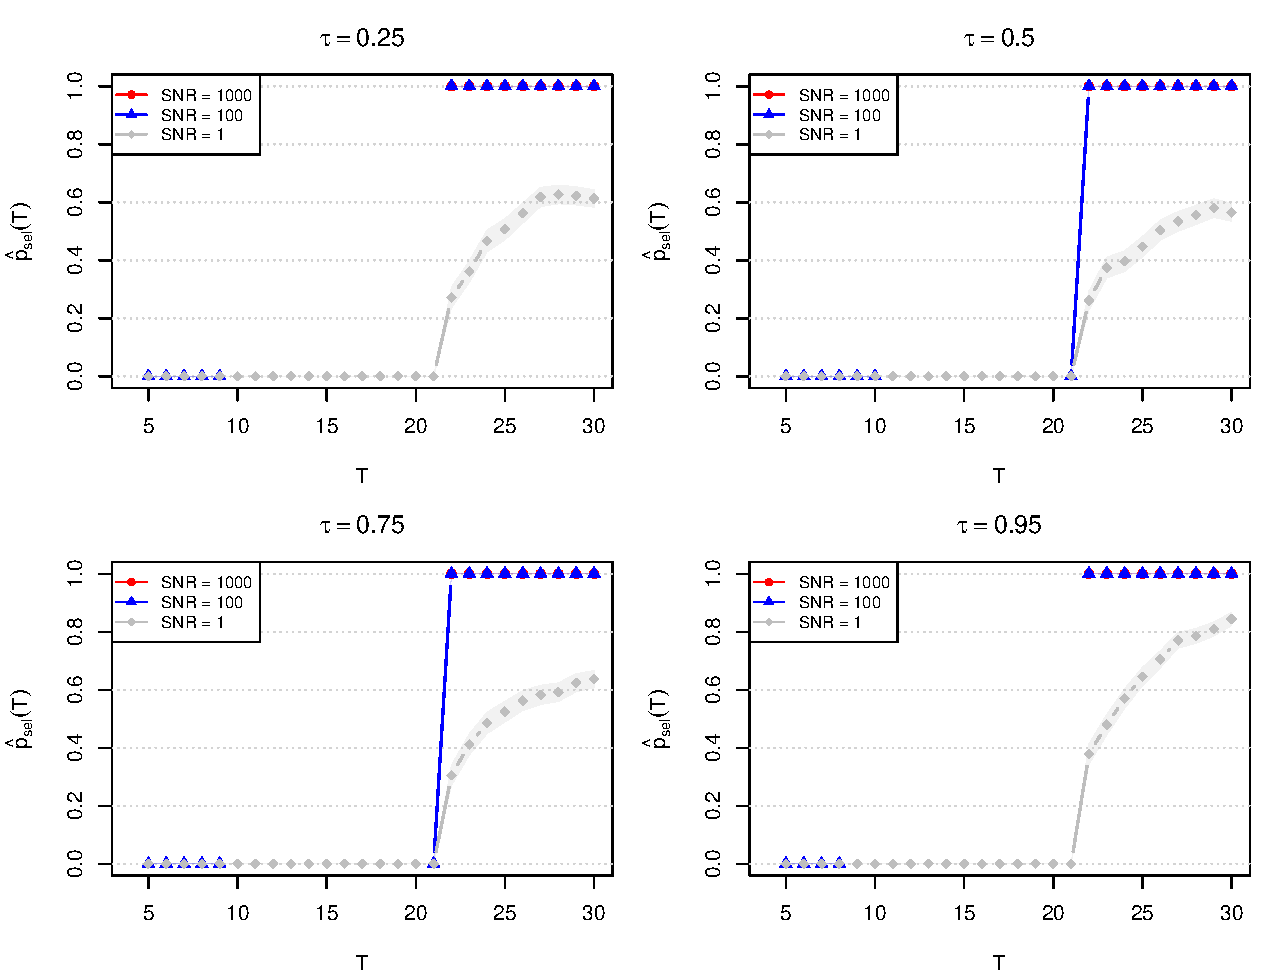
\includegraphics[width=0.93\textwidth]{monte-carlo-coverage-selected.pdf}
\caption{Empirical coverage $\widehat p^{\,\rm sel}_M(T)$ of the selected interval versus the horizon $T$ ($M=1000$), one panel per $\tau$ and one curve per SNR; the true peak is $L=22$.}
\label{fig:cov}
\end{figure}

\begin{table}[t]
\centering\small
\caption{Selection rate, empirical coverage and mean width at $T=30$ ($M=1000$).}
\label{tab:mc}
\begin{tabular}{cccccc}
\toprule
$\tau$ & SNR & $\widehat q_M(30)$ & $\widehat p^{\,\rm sel}_M(30)$ & $\widehat p^{\,\rm all}_M(30)$ & Mean width\\
\midrule
0.25 & 1000 & 1.000 & 1.000 & 1.000 & 18.70\\
0.25 & 100  & 1.000 & 1.000 & 1.000 & 12.66\\
0.25 & 1    & 0.998 & 0.613 & 0.612 & 5.62\\
\midrule
0.50 & 1000 & 1.000 & 1.000 & 1.000 & 18.26\\
0.50 & 100  & 1.000 & 1.000 & 1.000 & 11.98\\
0.50 & 1    & 0.996 & 0.565 & 0.563 & 5.49\\
\midrule
0.75 & 1000 & 1.000 & 1.000 & 1.000 & 18.79\\
0.75 & 100  & 1.000 & 1.000 & 1.000 & 12.72\\
0.75 & 1    & 0.996 & 0.637 & 0.634 & 5.30\\
\midrule
0.95 & 1000 & 1.000 & 1.000 & 1.000 & 19.66\\
0.95 & 100  & 1.000 & 1.000 & 1.000 & 14.20\\
0.95 & 1    & 1.000 & 0.844 & 0.844 & 5.75\\
\bottomrule
\end{tabular}
\end{table}

The results depend strongly on the SNR (Figure~\ref{fig:cov}, Table~\ref{tab:mc}). At SNR $=1000$ no interval is selected for $T<22$, and from $T=22$ onward both the selection rate and the coverage equal one. At SNR $=100$, selection is rare at some early horizons, but from $T=23$ onward every trajectory yields an interval that contains $L$. At SNR $=1$, intervals may be selected before $T=22$, but in our simulations none of them contains $L$; at $T=22$ the coverage among selected intervals is only about $0.26$--$0.38$, and it rises with $T$ to $0.57$--$0.84$ at $T=30$, depending on $\tau$ (best for $\tau=0.95$). Since the selection rate at $T=30$ is at least $0.996$, the low coverage at SNR $=1$ is not explained by failures to select. Note also that the perfect coverage at high and moderate SNR comes with wide intervals (mean width $12$--$20$ on a horizon of $30$), whereas the low-SNR intervals are narrow (about $5$--$6$) but often miss $L$. These are empirical coverage rates for this design, not a theoretical guarantee.

\section{Application to COVID-19 case counts}
We apply the procedure to daily confirmed cases in China (22 January--22 March 2020; JHU CSSE), France and Germany (ECDC), for $\tau\in\{0.25,0.5,0.75,0.95\}$. Because the observed peak $L$ is known retrospectively in each series, the candidates can be evaluated ex post: among those with $T^{(k)}_{\rm entry}<L<T^{(k)}_{\rm exit}$ we report the narrowest (this uses $L$ and is not part of the operational rule). Table~\ref{tab:covid} gives the resulting windows.

\begin{table}[t]
\centering\small
\caption{Retrospectively selected windows $(T_{\rm entry},T_{\rm exit})$ strictly containing the observed peak $L$; ``--'' means no candidate contains $L$.}
\label{tab:covid}
\begin{tabular}{lcccccc}
\toprule
Country & $L$ & $\tau=0.25$ & $\tau=0.50$ & $\tau=0.75$ & $\tau=0.95$\\
\midrule
China   & 22 & (15,26) & (15,24) & --      & (13,26)\\
France  & 78 & (72,79) & (73,82) & (70,79) & (70,80)\\
Germany & 61 & (60,62) & --      & --      & (56,63)\\
\bottomrule
\end{tabular}
\end{table}

For France, all four quantile levels give a window containing the peak, with widths between 7 and 10. For China the windows are $(15,24)$ at $\tau=0.5$, close to the window $(14,25)$ obtained by \citet{Der25} under the least-absolute-deviation criterion, while $\tau=0.75$ yields no containing candidate. For Germany only $\tau=0.25$ and $\tau=0.95$ do. The window therefore depends on the quantile level, and a containing window is not always available.

\section{Conclusion and perspectives}
Quantile regression with $\tau$-aligned asymmetric Laplace noise gives a unified criterion for peak-location estimation, and the oscillation-based entry--exit construction yields a data-driven interval for $L$ that is computed without knowledge of $L$. Simulation shows that its coverage is excellent but costly in width at high and moderate SNR, and limited at low SNR. Open questions are a theoretical coverage result (or a calibration of the selection rule to reach a target level), repeating the study across other peak locations and widths, and applying it to environmental series such as pollution or energy-demand peaks.

\bibliography{references}

\end{document}
